\subsection{Performance}\label{subsec:IO_Subsystem_Performance}
I/O is a major factor in system performance.
\begin{itemize}[noitemsep]
\item It places heavy demands on the CPU to execute \nameref{def:Device_Driver} code and to schedule \nameref{def:Process}es fairly and efficiently as they block and unblock.
  \begin{itemize}[noitemsep]
  \item The resulting \nameref{def:Context_Switch}es stress the CPU and its hardware caches.
\end{itemize}
\item I/O exposes inefficiencies in the \nameref{def:Interrupt_Handler} mechanisms in the \nameref{def:Kernel}.
\item I/O loads down the memory bus during data copies between \nameref{def:Controller}s and \nameref{def:Physical_Memory} and again during copies between kernel buffers and application data space.
\end{itemize}

Coping gracefully with all these demands is one of the major concerns of the OS designer/architect.

Interrupt handling is a relatively expensive task.
Each interrupt causes the system to perform a state change, to execute the interrupt handler, and then to restore state.
Network traffic can also cause a high context-switch rate (see \Cref{fig:Intercomputer_Communications}).

\begin{figure}[h!tbp]
  \centering
  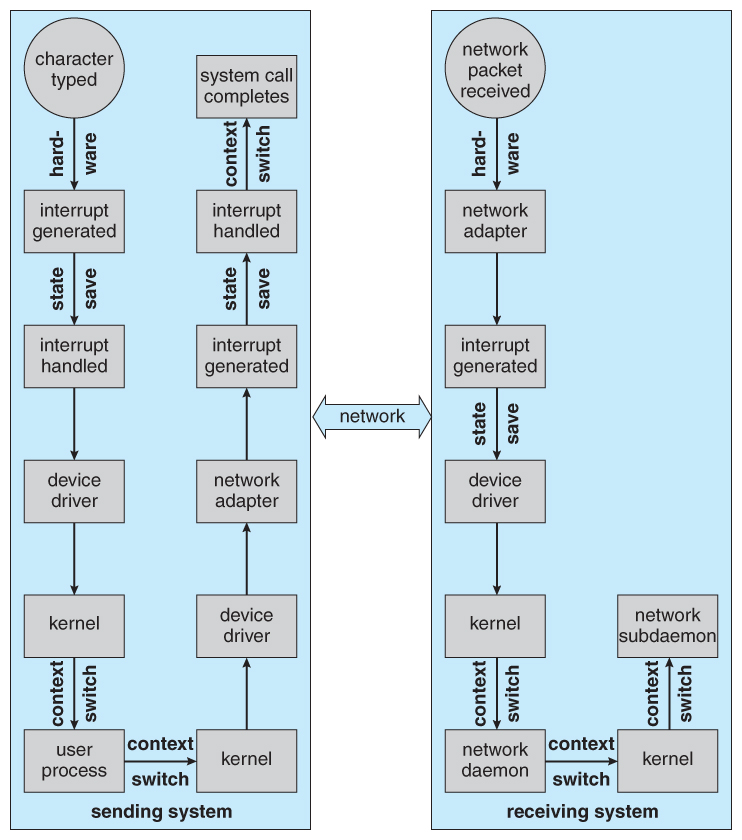
\includegraphics[scale=1.00]{./Drawings/EDAF35-Operating_Systems/Intercomputer_Communications.jpg}
  \caption{Intercomputer Communications}
  \label{fig:Intercomputer_Communications}
\end{figure}

To help alleviate the problems of network-based interrupts:
\begin{itemize}[noitemsep]
\item Reimplemented certain \nameref{def:Daemon}s using in-kernel threads.
\item Other systems use separate front-end processors for terminal I/O to reduce the interrupt burden on the main CPU.\@
  \begin{itemize}[noitemsep]
  \item For instance, a terminal concentrator can multiplex the traffic from hundreds of remote terminals into one port on a large computer.
  \end{itemize}
\item An I/O channel is a dedicated, special-purpose CPU found in mainframes and in other high-end systems.
  \begin{itemize}[noitemsep]
  \item The job of a channel is to offload I/O work from the main CPU.\@
  \item The idea is that the channels keep the data flowing smoothly, while the main CPU remains free to process the data.
  \end{itemize}
\end{itemize}

Like device controllers and DMA controllers found in smaller computers, a channel can process more general and sophisticated programs, so channels can be tuned for particular workloads.

\subsubsection{Improving Efficiency}\label{subsubsec:Improve_IO_Subsystem_Performance}
\begin{itemize}[noitemsep]
\item Reduce the number of \nameref{def:Context_Switch}es.
\item Reduce the number of times that data must be copied in memory while passing between device and application.
\item Reduce the frequency of \nameref{def:Interrupt}s by using:
  \begin{itemize}[noitemsep]
  \item Large transfers.
  \item Smart controllers.
  \item Polling (if busy waiting can be minimized).
  \end{itemize}
\item Increase concurrency by using DMA-knowledgeable controllers or channels to offload simple data copying from the CPU.\@
\item Move processing primitives into hardware, to allow their operation in device controllers to be concurrent with CPU and bus operation.
\item Balance CPU, memory subsystem, bus, and I/O performance.
  \begin{itemize}[noitemsep]
  \item An overload in any one area will cause idleness in others.
  \end{itemize}
\end{itemize}

%%% Local Variables:
%%% mode: latex
%%% TeX-master: "../../EDAF35-Operating_Systems-Reference_Sheet"
%%% End:
